\documentclass[14pt]{extbook}
\usepackage{multicol, enumerate, enumitem, hyperref, color, soul, setspace, parskip, fancyhdr} %General Packages
\usepackage{amssymb, amsthm, amsmath, latexsym, units, mathtools} %Math Packages
\everymath{\displaystyle} %All math in Display Style
% Packages with additional options
\usepackage[headsep=0.5cm,headheight=12pt, left=1 in,right= 1 in,top= 1 in,bottom= 1 in]{geometry}
\usepackage[usenames,dvipsnames]{xcolor}
\usepackage{dashrule}  % Package to use the command below to create lines between items
\newcommand{\litem}[1]{\item#1\hspace*{-1cm}\rule{\textwidth}{0.4pt}}
\pagestyle{fancy}
\lhead{Progress Quiz 6}
\chead{}
\rhead{Version C}
\lfoot{1430-1829}
\cfoot{}
\rfoot{test}
\begin{document}

\begin{enumerate}
\litem{
First, find the equation of the line containing the two points below. Then, write the equation as $ y=mx+b $ and choose the intervals that contain $m$ and $b$.\[ (-7, -6) \text{ and } (8, 4) \]\begin{enumerate}[label=\Alph*.]
\item \( m \in [-0.1, 1.2] \hspace*{3mm} b \in [-4.35, -3.6] \)
\item \( m \in [-0.1, 1.2] \hspace*{3mm} b \in [0.62, 1.27] \)
\item \( m \in [-0.1, 1.2] \hspace*{3mm} b \in [-1.51, -1.16] \)
\item \( m \in [-2.5, -0.5] \hspace*{3mm} b \in [9.3, 9.44] \)
\item \( m \in [-0.1, 1.2] \hspace*{3mm} b \in [1.29, 1.82] \)

\end{enumerate} }
\litem{
Solve the linear equation below. Then, choose the interval that contains the solution.\[ \frac{5x + 7}{6} - \frac{3x + 7}{3} = \frac{9x + 8}{5} \]\begin{enumerate}[label=\Alph*.]
\item \( x \in [-4.29, -3.52] \)
\item \( x \in [-0.78, 0.67] \)
\item \( x \in [0.86, 1.32] \)
\item \( x \in [-1.93, -1.19] \)
\item \( \text{There are no real solutions.} \)

\end{enumerate} }
\litem{
First, find the equation of the line containing the two points below. Then, write the equation as $ y=mx+b $ and choose the intervals that contain $m$ and $b$.\[ (-8, -2) \text{ and } (4, 5) \]\begin{enumerate}[label=\Alph*.]
\item \( m \in [-0.42, 3.58] \hspace*{3mm} b \in [0.71, 1.46] \)
\item \( m \in [-0.42, 3.58] \hspace*{3mm} b \in [2.12, 2.74] \)
\item \( m \in [-6.58, 0.42] \hspace*{3mm} b \in [6.99, 8.23] \)
\item \( m \in [-0.42, 3.58] \hspace*{3mm} b \in [4.97, 6.06] \)
\item \( m \in [-0.42, 3.58] \hspace*{3mm} b \in [-2.81, -1.78] \)

\end{enumerate} }
\litem{
Write the equation of the line in the graph below in Standard form $Ax+By=C$. Then, choose the intervals that contain $A, B, \text{ and } C$.
\begin{center}
    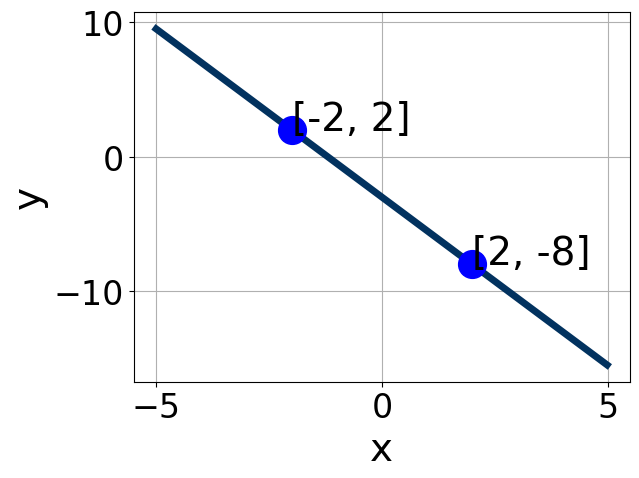
\includegraphics[width=0.5\textwidth]{../Figures/linearGraphToStandardC.png}
\end{center}
\begin{enumerate}[label=\Alph*.]
\item \( A \in [-4.75, 2.25], \hspace{3mm} B \in [-2.6, -0.2], \text{ and } \hspace{3mm} C \in [0, 4] \)
\item \( A \in [5, 9], \hspace{3mm} B \in [-4.9, -2.5], \text{ and } \hspace{3mm} C \in [8, 12] \)
\item \( A \in [5, 9], \hspace{3mm} B \in [1.6, 5.3], \text{ and } \hspace{3mm} C \in [-15, -3] \)
\item \( A \in [-4.75, 2.25], \hspace{3mm} B \in [-0.7, 1.4], \text{ and } \hspace{3mm} C \in [-7, 0] \)
\item \( A \in [-7, -2], \hspace{3mm} B \in [-4.9, -2.5], \text{ and } \hspace{3mm} C \in [8, 12] \)

\end{enumerate} }
\litem{
Solve the equation below. Then, choose the interval that contains the solution.\[ -4(-14x -5) = -3(10x + 9) \]\begin{enumerate}[label=\Alph*.]
\item \( x \in [0.17, 0.3] \)
\item \( x \in [-0.76, -0.39] \)
\item \( x \in [-0.01, 0.13] \)
\item \( x \in [-0.12, 0.02] \)
\item \( \text{There are no real solutions.} \)

\end{enumerate} }
\litem{
Solve the linear equation below. Then, choose the interval that contains the solution.\[ \frac{7x + 4}{3} - \frac{6x + 9}{2} = \frac{6x + 9}{8} \]\begin{enumerate}[label=\Alph*.]
\item \( x \in [3.32, 5.32] \)
\item \( x \in [-4.03, -2.03] \)
\item \( x \in [-1.86, 1.14] \)
\item \( x \in [-11.88, -4.88] \)
\item \( \text{There are no real solutions.} \)

\end{enumerate} }
\litem{
Solve the equation below. Then, choose the interval that contains the solution.\[ -4(15x + 7) = -9(14x + 3) \]\begin{enumerate}[label=\Alph*.]
\item \( x \in [-0.92, -0.66] \)
\item \( x \in [0.48, 0.97] \)
\item \( x \in [-0.08, 0.11] \)
\item \( x \in [-0.62, -0.25] \)
\item \( \text{There are no real solutions.} \)

\end{enumerate} }
\litem{
Find the equation of the line described below. Write the linear equation as $ y=mx+b $ and choose the intervals that contain $m$ and $b$.\[ \text{Perpendicular to } 8 x + 9 y = 4 \text{ and passing through the point } (3, 10). \]\begin{enumerate}[label=\Alph*.]
\item \( m \in [1.03, 1.25] \hspace*{3mm} b \in [-6.78, -6.24] \)
\item \( m \in [-1.17, -1.05] \hspace*{3mm} b \in [13.26, 13.46] \)
\item \( m \in [1.03, 1.25] \hspace*{3mm} b \in [6.67, 7.04] \)
\item \( m \in [0.8, 1.01] \hspace*{3mm} b \in [6.62, 6.88] \)
\item \( m \in [1.03, 1.25] \hspace*{3mm} b \in [6.62, 6.88] \)

\end{enumerate} }
\litem{
Write the equation of the line in the graph below in Standard form $Ax+By=C$. Then, choose the intervals that contain $A, B, \text{ and } C$.
\begin{center}
    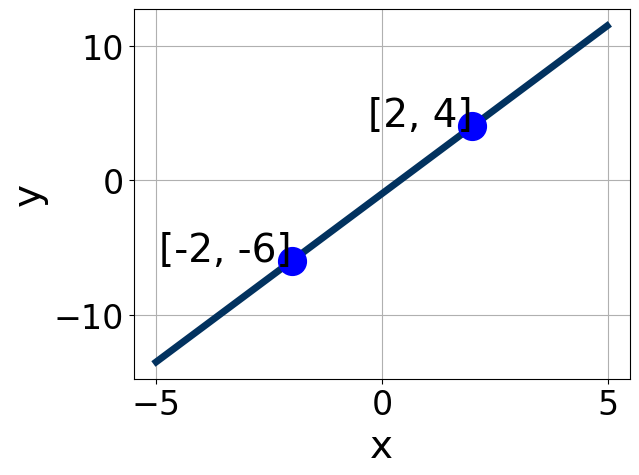
\includegraphics[width=0.5\textwidth]{../Figures/linearGraphToStandardCopyC.png}
\end{center}
\begin{enumerate}[label=\Alph*.]
\item \( A \in [2, 3.7], \hspace{3mm} B \in [-5.25, -3.75], \text{ and } \hspace{3mm} C \in [20, 24] \)
\item \( A \in [-1.1, 2.3], \hspace{3mm} B \in [-0.06, 1.94], \text{ and } \hspace{3mm} C \in [-5, 2] \)
\item \( A \in [2, 3.7], \hspace{3mm} B \in [4.56, 6.16], \text{ and } \hspace{3mm} C \in [-20, -19] \)
\item \( A \in [-1.1, 2.3], \hspace{3mm} B \in [-1.41, -0.72], \text{ and } \hspace{3mm} C \in [4, 6] \)
\item \( A \in [-5.3, -2.3], \hspace{3mm} B \in [-5.25, -3.75], \text{ and } \hspace{3mm} C \in [20, 24] \)

\end{enumerate} }
\litem{
Find the equation of the line described below. Write the linear equation as $ y=mx+b $ and choose the intervals that contain $m$ and $b$.\[ \text{Perpendicular to } 9 x + 7 y = 14 \text{ and passing through the point } (-7, 7). \]\begin{enumerate}[label=\Alph*.]
\item \( m \in [0.73, 1.14] \hspace*{3mm} b \in [-13.44, -8.44] \)
\item \( m \in [-0.9, -0.36] \hspace*{3mm} b \in [-3.44, 2.56] \)
\item \( m \in [1.13, 1.51] \hspace*{3mm} b \in [10.44, 13.44] \)
\item \( m \in [0.73, 1.14] \hspace*{3mm} b \in [10.44, 13.44] \)
\item \( m \in [0.73, 1.14] \hspace*{3mm} b \in [14, 18] \)

\end{enumerate} }
\end{enumerate}

\end{document}